% {Youssouph Cissokho}
\newpage

\section{Applications à des problèmes réels}
Dans cette section, nous fournirons une comparaison expérimentale de quelques méthodes classiques  mentionnées ci-haut  pour tester et comparer les techniques de détection des valeurs aberrantes proposées sur des données réelles. \newl
\textbf{a) Données de compagnies aériennes:} Comprend les informations sur tous les vols intérieurs aux USA  en 2019, tels que l'heure de départ, l'heure d'arrivée, l'aéroport d'origine, l'aéroport de destination, etc.  Il est question d’analyser les retards accusés aux  départs et/ou à l’arrivée des vols. En effet, un vol est considéré comme à “l’heure”  \textbf{s’il arrive moins de 15 minutes plus tard que l'heure indiquée} dans les systèmes de réservation informatisés (CRS) du transporteur. Par conséquent, les anomalies sont les vols qui accusent des retards chroniques. Pour ce faire,  un échantillon de 500 vols au départ de l’aéroport de Chicago O’Hare (ORD) est extrait et on calcule les délais de retards moyens aux aéroports. Le délai moyen d’arrivée est calculé sur tous les vols atterrissant à un aéroport donné.\textbf{ Les anomalies sont donc les aéroports qui affichent des délais moyens inhabituels.}
%\begin{figure}[H]
%\centering
%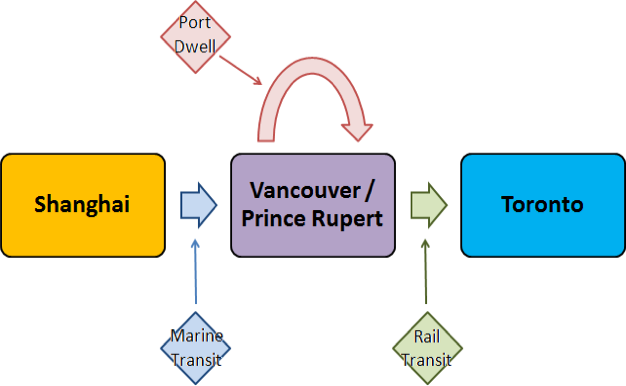
\includegraphics[width=0.5\textwidth]{Images/mmsc.png}
%\caption{\small Multi-modal supply chain.} %\label{fig:mmsc}
%\end{figure}
\begin{figure}[H]
    \centering
    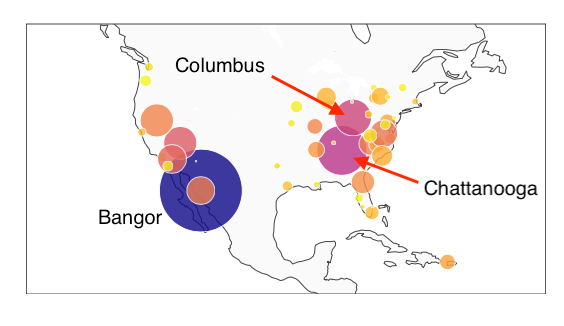
\includegraphics[width=.50\textwidth]{ADOA/Images/vols1.png}
    %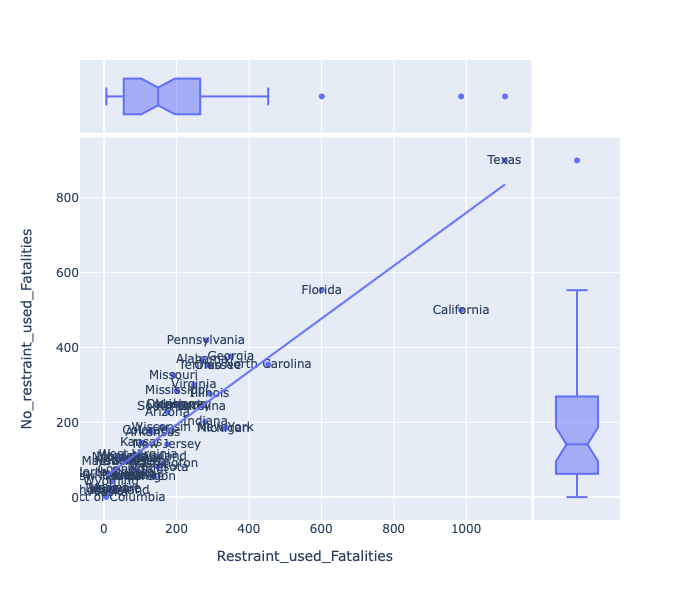
\includegraphics[width=.40\textwidth]{ADOA/Images/Fatal1.png}
    \caption{Nuage de points des retards accusés à l'arrivée sur la carte avec comme taille des boules la variable ARR\_DELAY.}%\hrule
    \label{fig20}
\end{figure}
\noindent La figure \ref{fig20}, montre les aéroports \textbf{Bangor, Chattanooga, Columbus,etc.} affichent des délais moyens inhabituels (trés élevés) et donc sont anormales. Quelques méthdes ont donc fait l'objet d'analyses détaillées, les résultats sont dans la figure \ref{fig21}
\begin{figure*}[t]
    \centering
    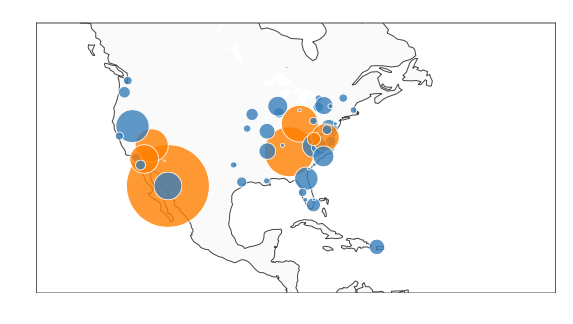
\includegraphics[width=.45\textwidth]{ADOA/Images/vol1PCA.png}
    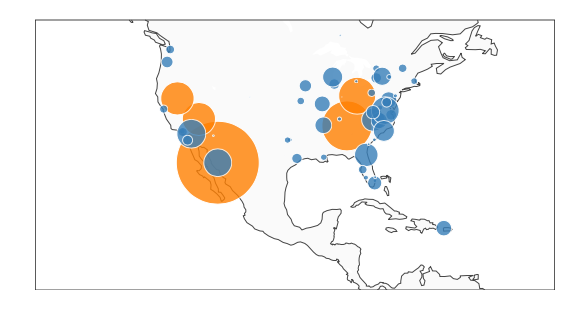
\includegraphics[width=.450\textwidth]{ADOA/Images/vols1KNN.png}\\
    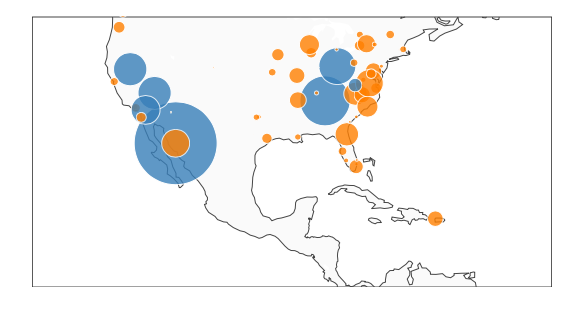
\includegraphics[width=.45\textwidth]{ADOA/Images/volsIsoFor.png}
    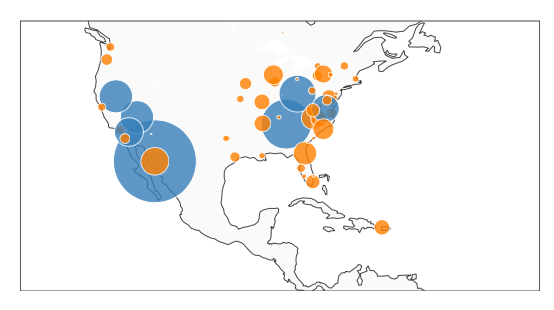
\includegraphics[width=.450\textwidth]{ADOA/Images/volsLOFpng.png}
    \caption{Aéroports détectés comme aberrants par PCA (en haut à gauche), KNN (en haut à droite), Isolation Forest (en bas à gauche) et LOF (en bas à droite)}%\hrule
    \label{fig21}
\end{figure*}\\
\textbf{Analyse des résultats:} 
Dans les figures \ref{fig21}, vous pouvez voir les aéroports aberrants tels que détectés par les différentes techniques. Les cercles bleus représentent les aéroports sans comportement aberrant, tandis que les cercles oranges représentent les aéroports avec un comportement aberrant pour (\textbf{PCA and KNN}). \textbf{Le délai moyen d'arrivée définit la taille des marqueurs}. Quelques aéroports sont systématiquement identifiés comme des points aberrants par toutes les techniques: l’aéroport de \textbf{Bangor, Columbus, Chattanooga et Las vegas}. Cependant, l’aéroport de \textbf{Bangor} est le plus gros complexe avec un très long retard à l’arrivée (141 minutes). Cet aéroport pourrait donc être candidat à une inspection plus poussée des processus et de l’infrastructure de l’aéroport ou encore des retards causés par de mauvaises conditions climatiques.\newl
\noindent\textbf{b) Accidents mortels:}
 est une donnèe qui représente les accidents mortels concernent uniquement les occupants de voitures de tourisme et de camionnettes aux États-Unis. Ces accidents impliquent toute activité susceptible de détourner l'attention d'une personne de la tâche principale de la conduite, comme envoyer des SMS, utiliser un téléphone portable, manger et boire, se toiletter, utiliser un système de navigation, régler la radio, etc. disponible  \href{https://www.bts.dot.gov/content/passenger-car-and-light-truck-occupants-killed-and-restraint-use}{\underline{ici}}. Une analyse visuelle de la Figure \ref{fig2}, montre qu'il y a des pays qui se distinguent des autres avec un nombre élevé d'accidents mortels dans ces pays. D'autre part, la boîte à moustaches, nous indique également que ces pays sont anormaux (aberrants), ces pays sont \textbf{Texas, california, Florida}. Une analyse plus approfondie est menée pour corroborer les résultats antérieurs. Ces méthodes sont \textbf{ KNN, PCA, LOF and Isolation Forest}. Pour ce faire, les variables sont normalisées afin d’éviter que celles qui ont des grandes échelles dominent les autres. Le resultat est présenté dans la Figure \ref{fig3}. 
\begin{figure}[H]
    \centering
    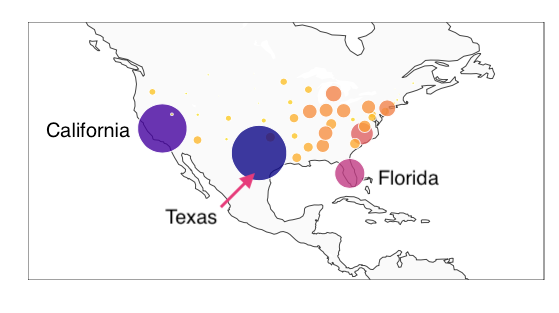
\includegraphics[width=.5\textwidth]{ADOA/Images/fat1png.png}
    %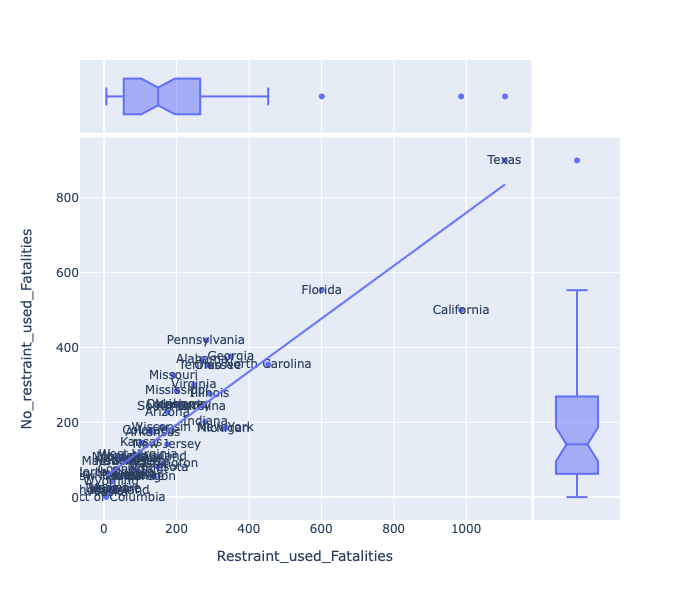
\includegraphics[width=.40\textwidth]{ADOA/Images/Fatal1.png}
    \caption{analyse de 2 composantes}%\hrule
    \label{fig2}
\end{figure}

 \begin{figure}[ht]
    \centering
    %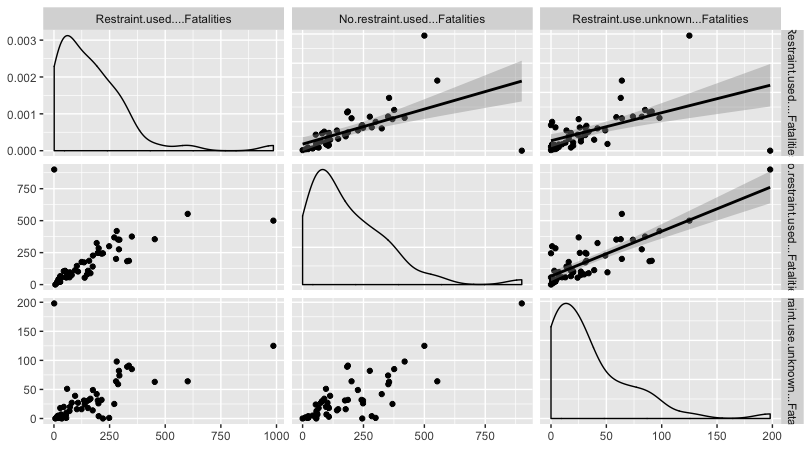
\includegraphics[width=.55\textwidth]{ADOA/Images/Fatal.png}
    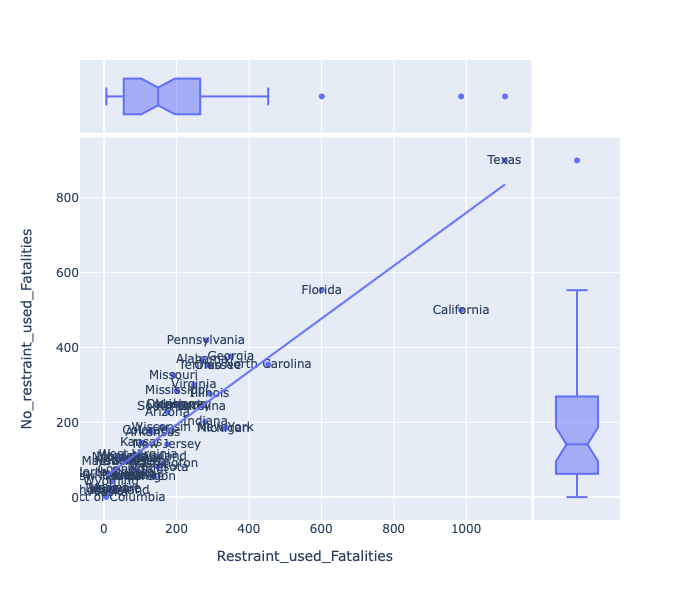
\includegraphics[width=.50\textwidth]{ADOA/Images/Fatal1.png}
    \caption{analyse de 2 composantes}%\hrule
    \label{fig2a}
\end{figure}

 \begin{figure*}[H]
    \centering
    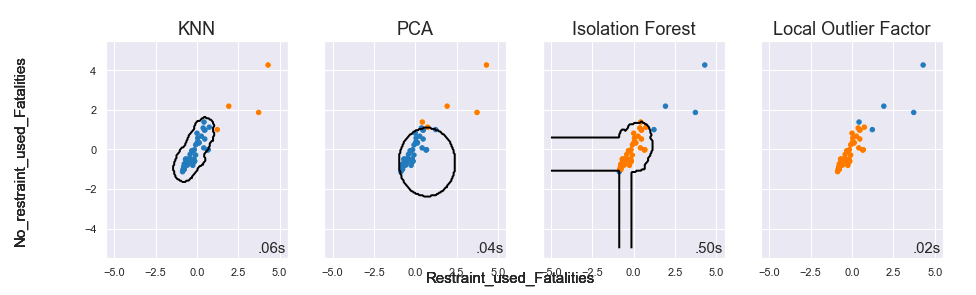
\includegraphics[width=1\textwidth]{ADOA/Images/Fatal11.png}
    \caption{Illustration des performences des méthodes: KNN, PCA, Isolation forest and LOF}%\hrule
    \label{fig3}
\end{figure*}
\vspace{2cm}

\begin{figure*}[t]
    \centering
    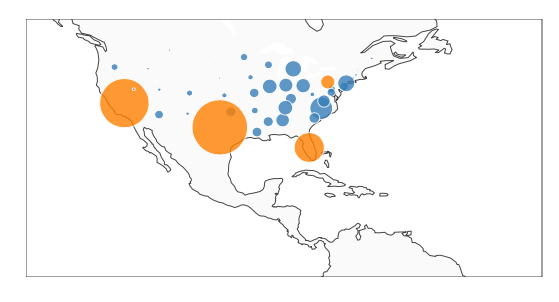
\includegraphics[width=.45\textwidth]{ADOA/Images/FatPCA.png}
    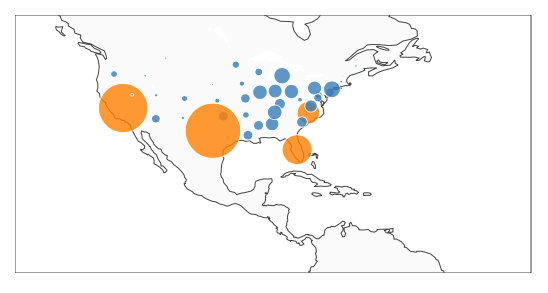
\includegraphics[width=.450\textwidth]{ADOA/Images/FatKNN.png}\\
    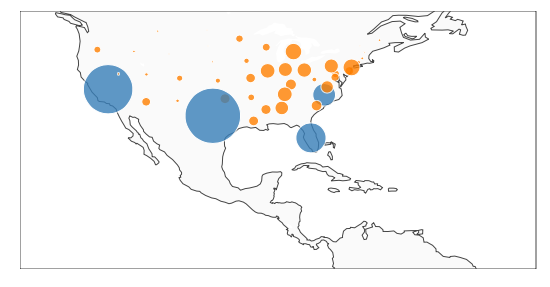
\includegraphics[width=.45\textwidth]{ADOA/Images/FatIsofore.png}
    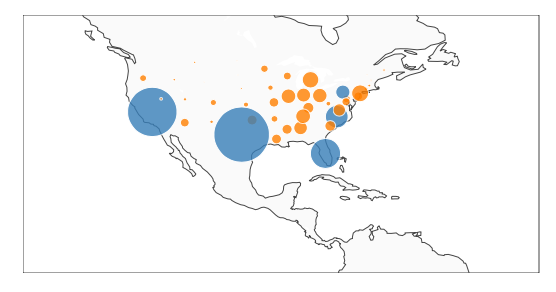
\includegraphics[width=.450\textwidth]{ADOA/Images/FatLOF.png}
    \caption{Villes détectées comme aberrantes par PCA (en haut à gauche), KNN (en haut à droite), Isolation Forest (en bas à gauche) et LOF (en bas à droite)}%\hrule
    \label{fig2b}
\end{figure*}

\newpage
\textbf{Global cities data set:} 
 C’est une donnée de dimension 68 $\times$ 32, les lignes représentent  68 capitales  et les colonnes représentent les caractéristiques  des ces capitales telles que pays, continent, population totale etc.   Il s’agit là d’une détection des valeurs aberrantes non supervisée car on ne connait pas les capitales qui ont des caractéristiques différentes des autres. L’objectif est de repérer les capitales qui ont des particularités différentes par rapport à certaines variables. Les variables suivantes:  Life.Expectancy.in.Years..Male., Life.Expectancy.in.Years..Female. ,Life.Expectancy, Air.Quality., City.Population..millions., Metro.Population..millions, City.Area..km2., Metro.Area..km2., ont été extraites puis normalisée avant de les passer aux algorithmes. La Figure\ref{fig6} Montre les résultats obtenus.
%\begin{figure*}[ht]
   % \centering
%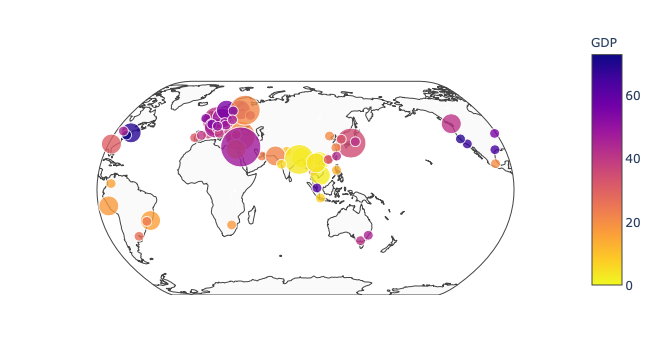
\includegraphics[width=1\textwidth]{ADOA/Images/Globbpng.png}
 %   \caption{Nuage de points de GPD sur la carte avec comme taille des boulesla variable gen.rating }%\hrule
%    \label{fig4}
%\end{figure*}

%Perhaps an image (see Figure~\ref{fig:Cities}?
%\begin{figure*}[t]
   % \centering
   % 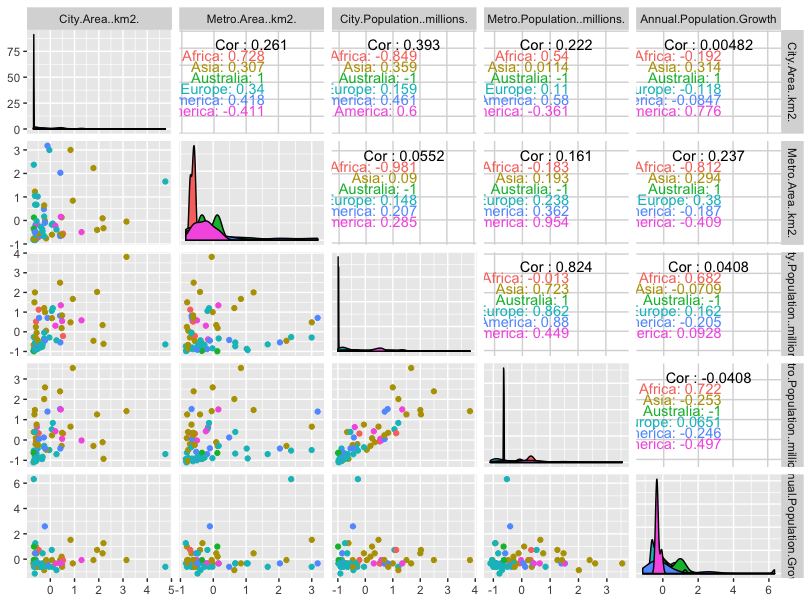
\includegraphics[width=\textwidth]{ADOA/Images/Corr1.png}
   % 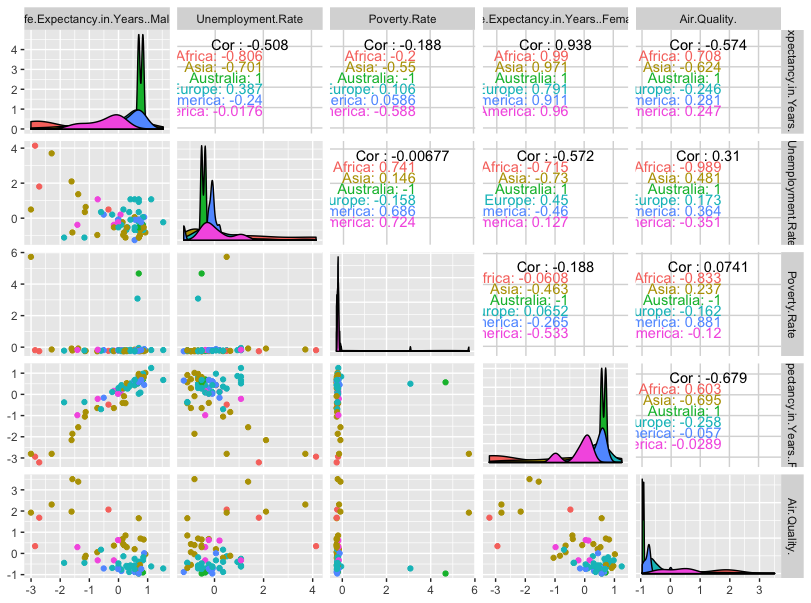
\includegraphics[width=\textwidth]{ADOA/Images/Corr2.png}
   % \caption{.}\hrule
   % \label{fig:Citiesbb}
%\end{figure*}
%%\begin{figure*}[t]
  %  \centering
 %   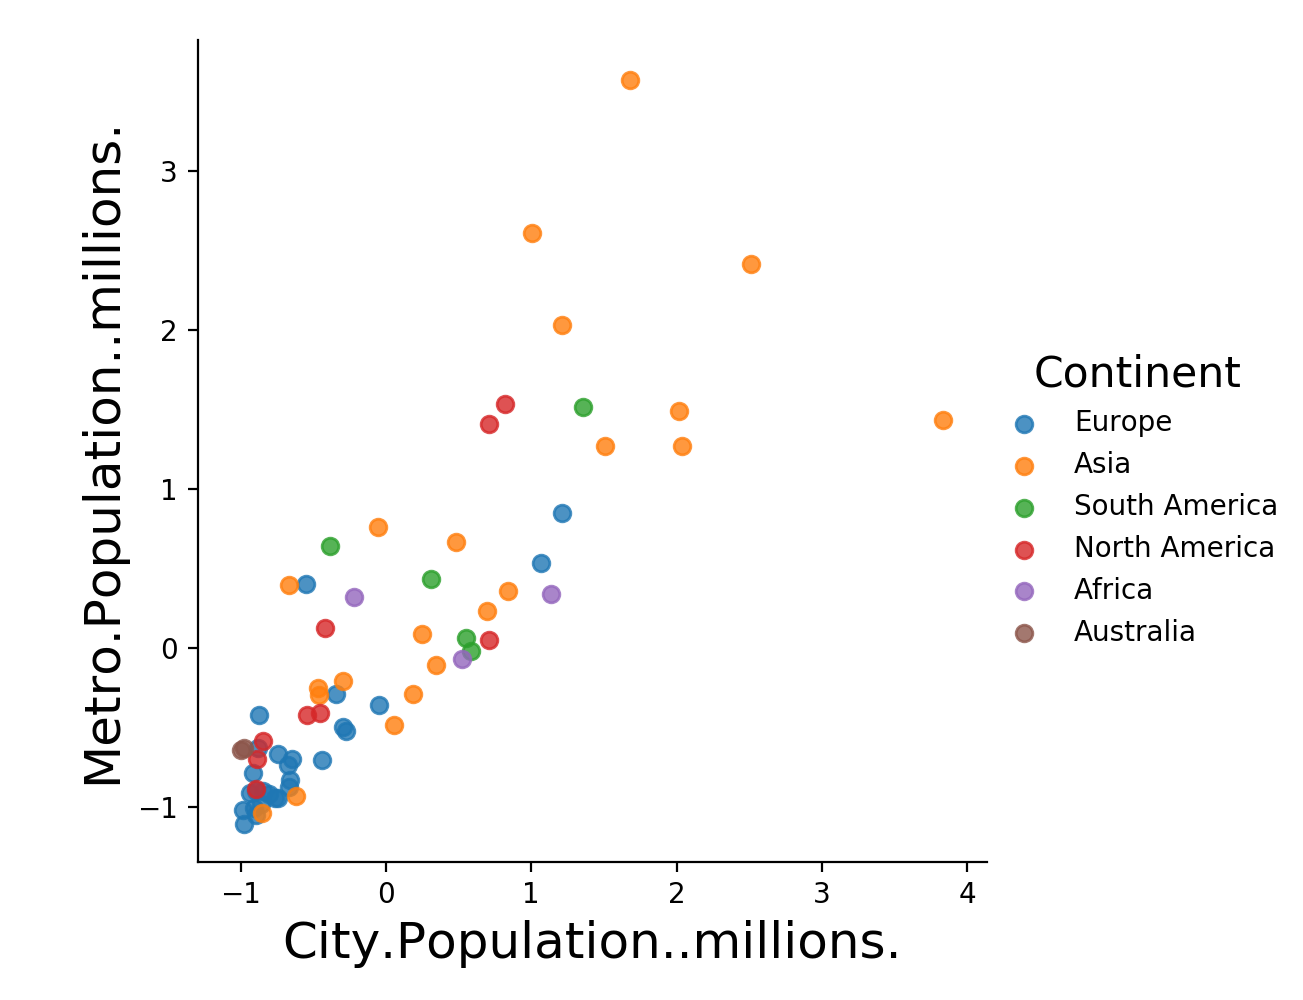
\includegraphics[width=.40\textwidth]{ADOA/Images/CityPopu.png}
 %   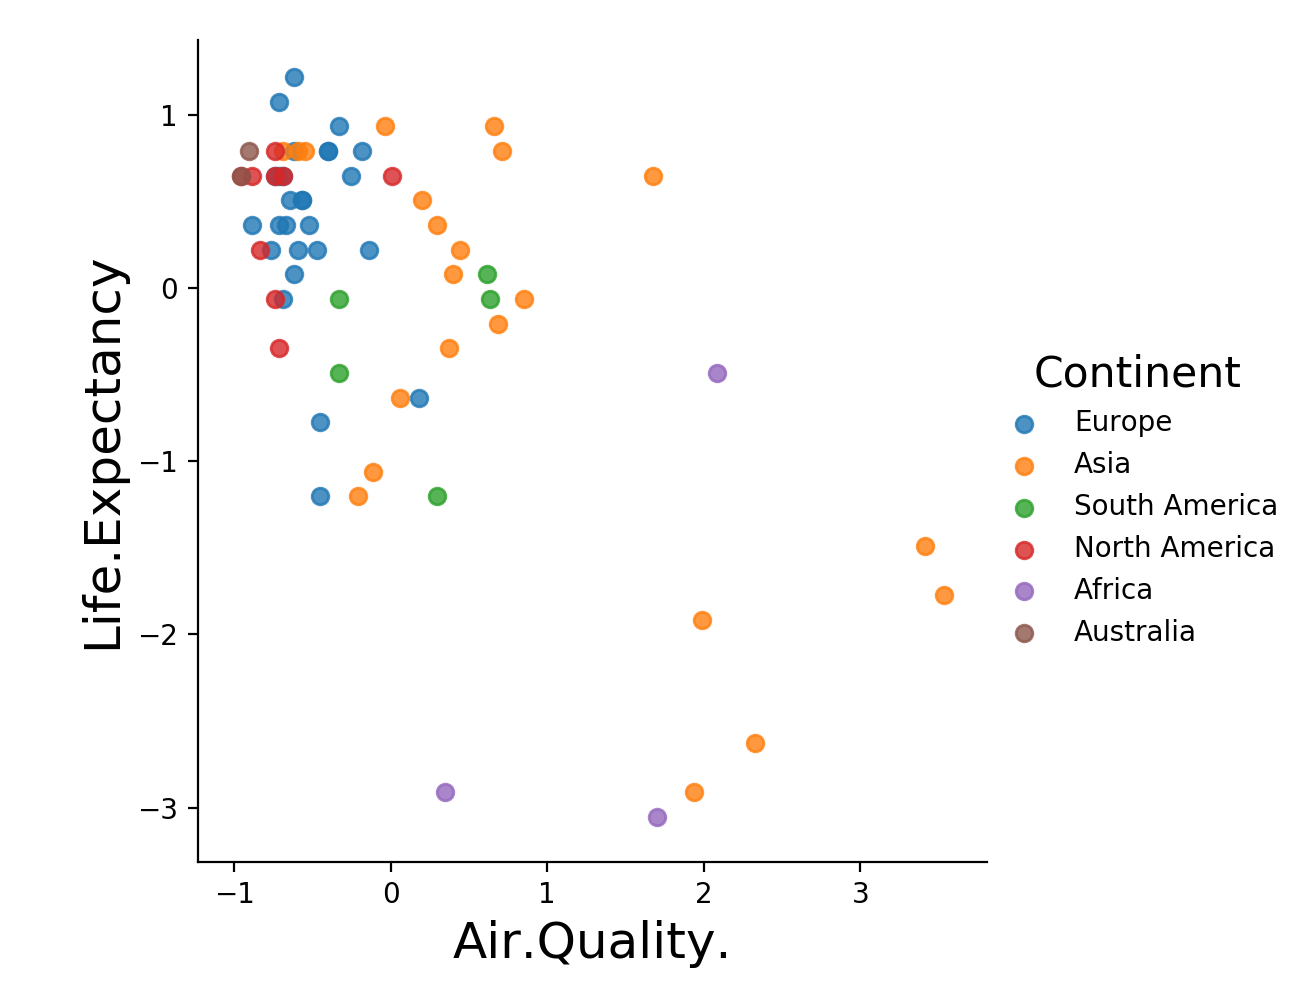
\includegraphics[width=.4\textwidth]{ADOA/Images/AirquaLifeExp.png}
 %   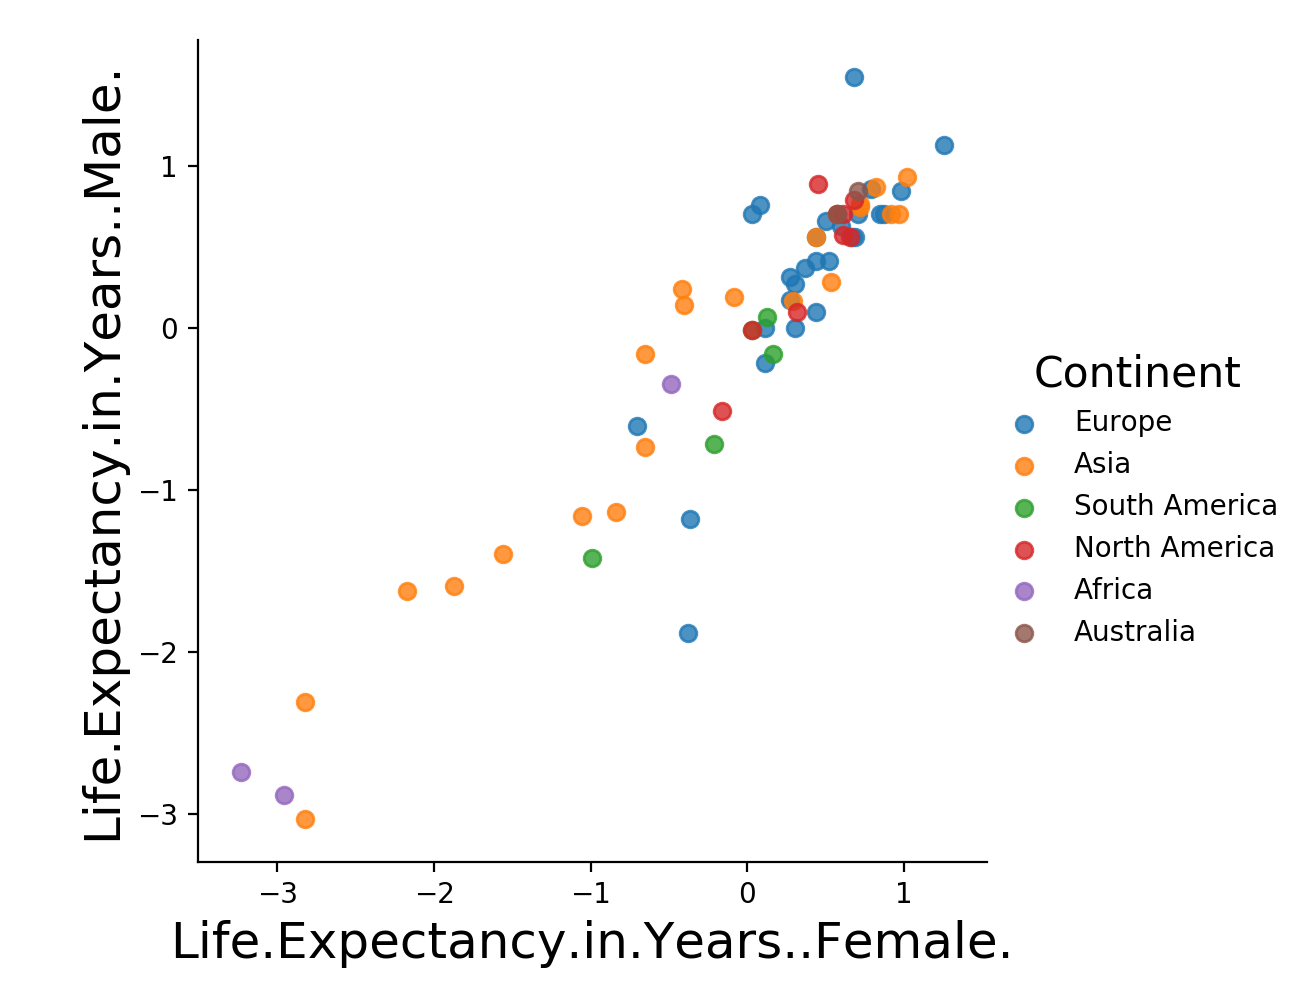
\includegraphics[width=.4\textwidth]{ADOA/Images/LifeExpMaleFemale.png} %
 %   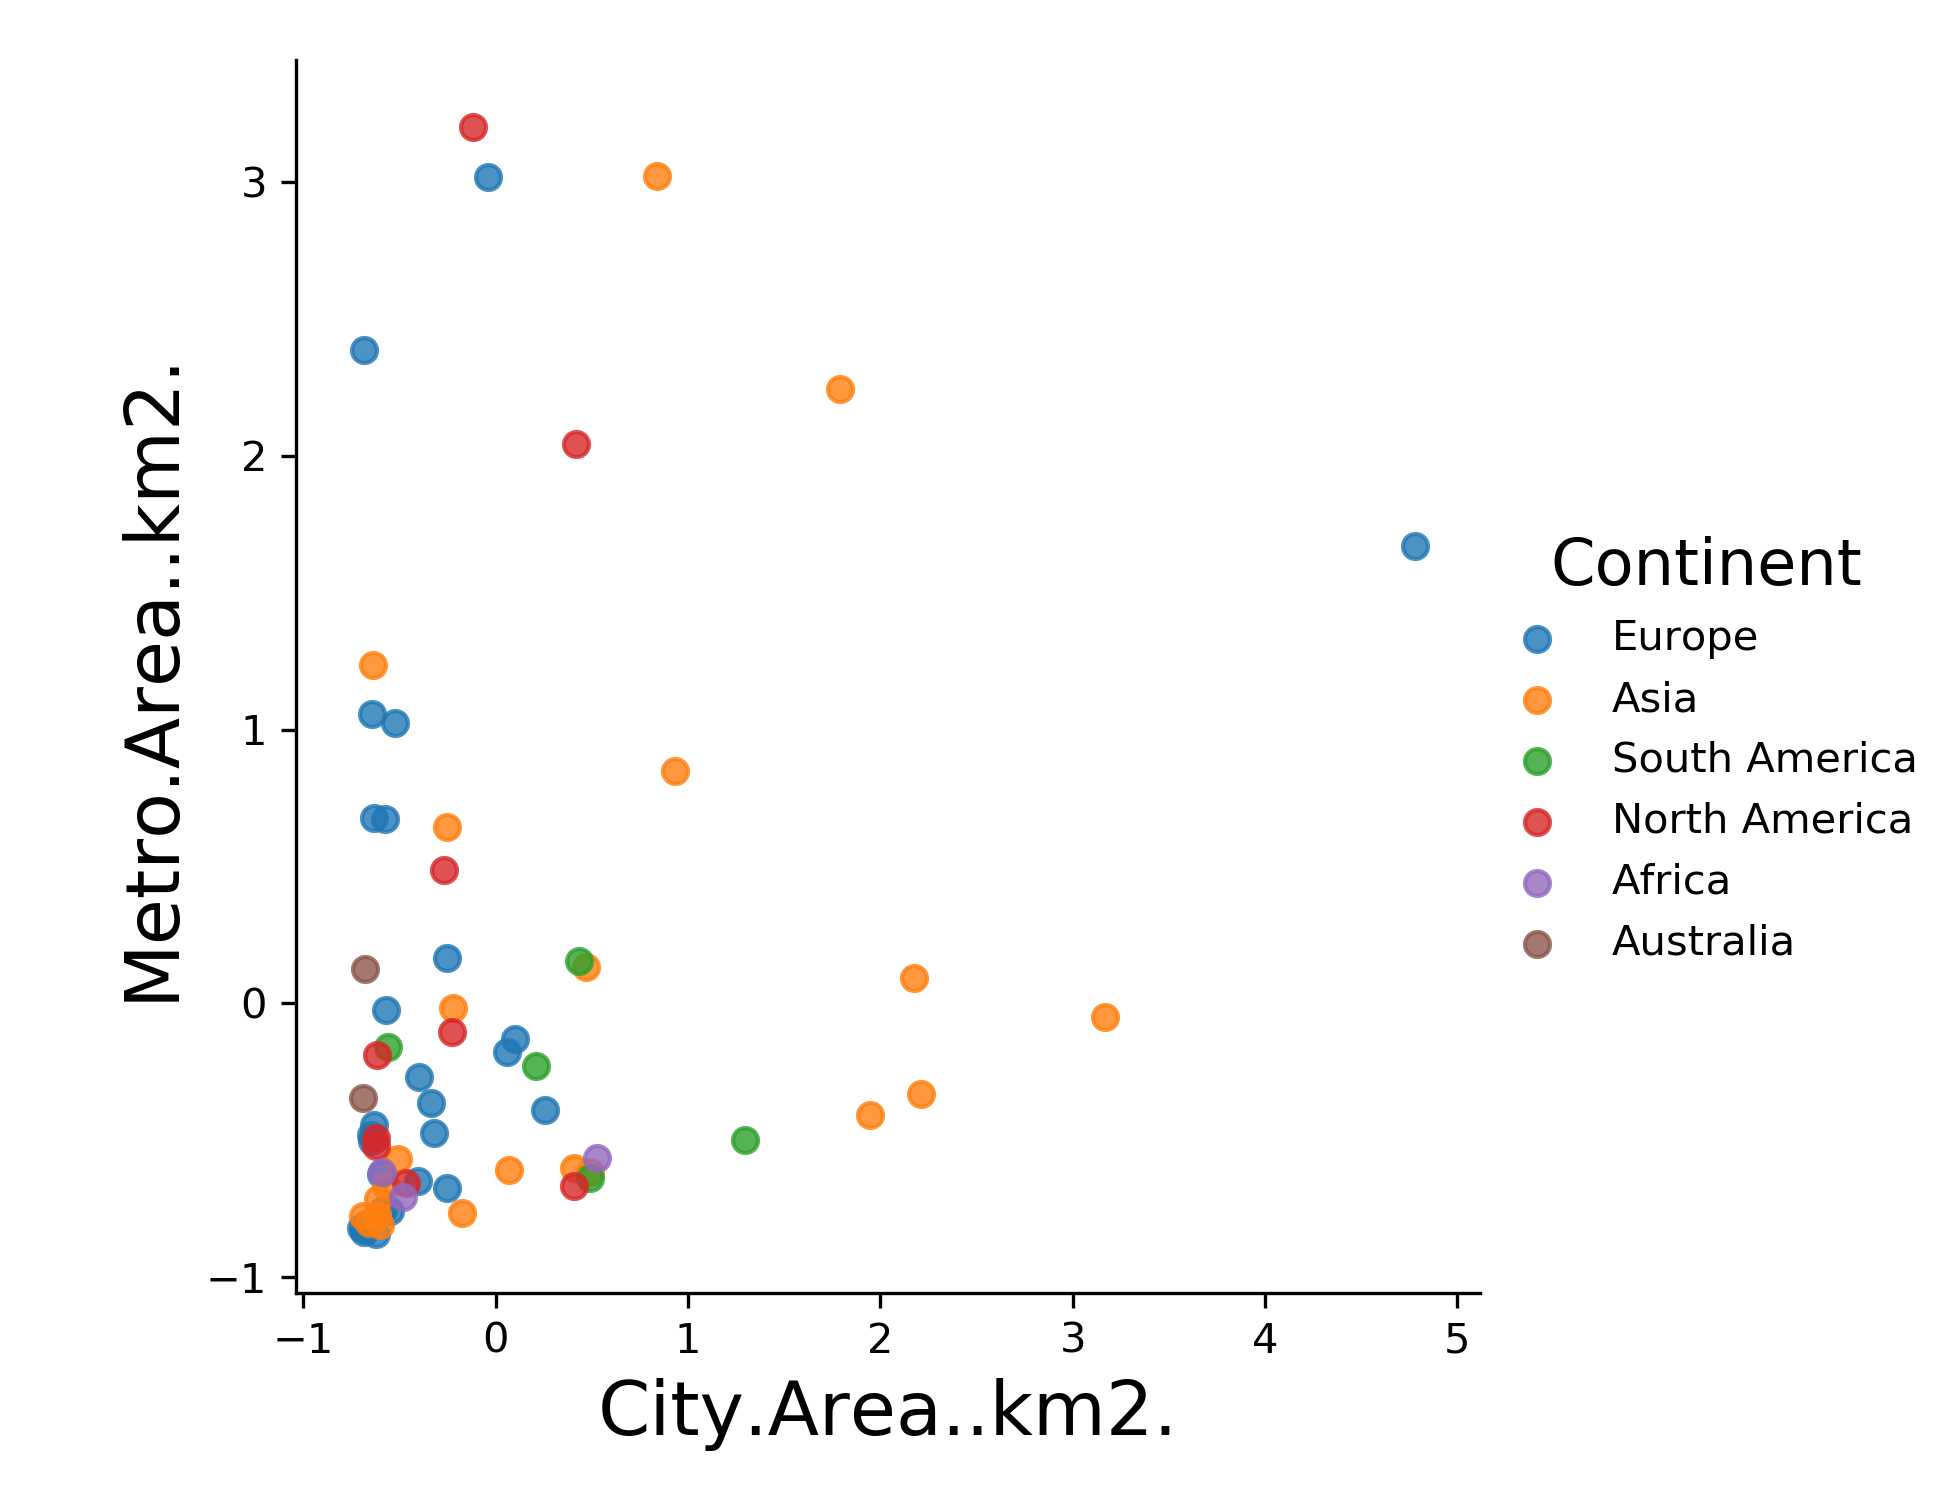
\includegraphics[width=.4\textwidth]{ADOA/Images/CityAreaMetro.png} 
  %  \caption{.}\hrule
 %  \label{fig:fig5}
%\end{figure*}
%%\begin{figure*}[t]
  %  \centering
  %  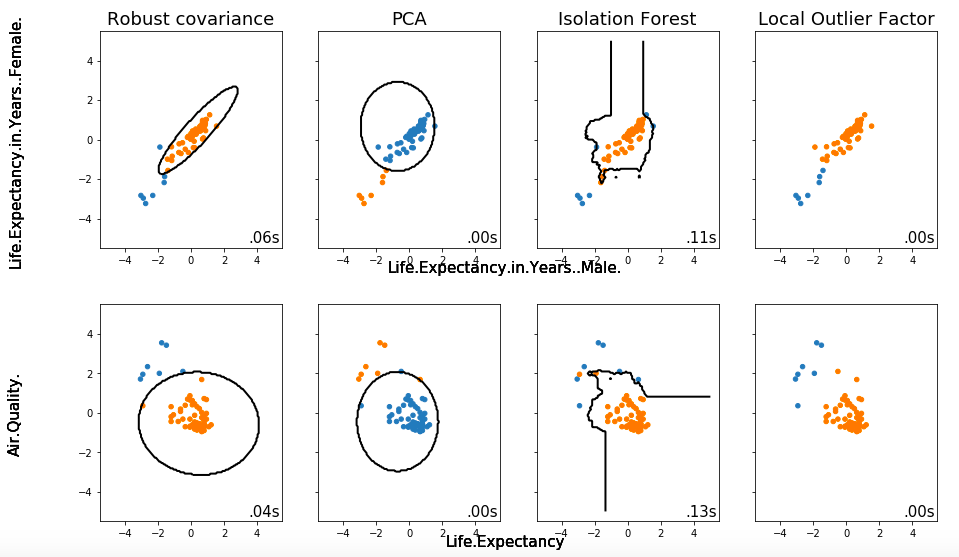
\includegraphics[width=\textwidth]{ADOA/Images/Allcomp1.png}
   %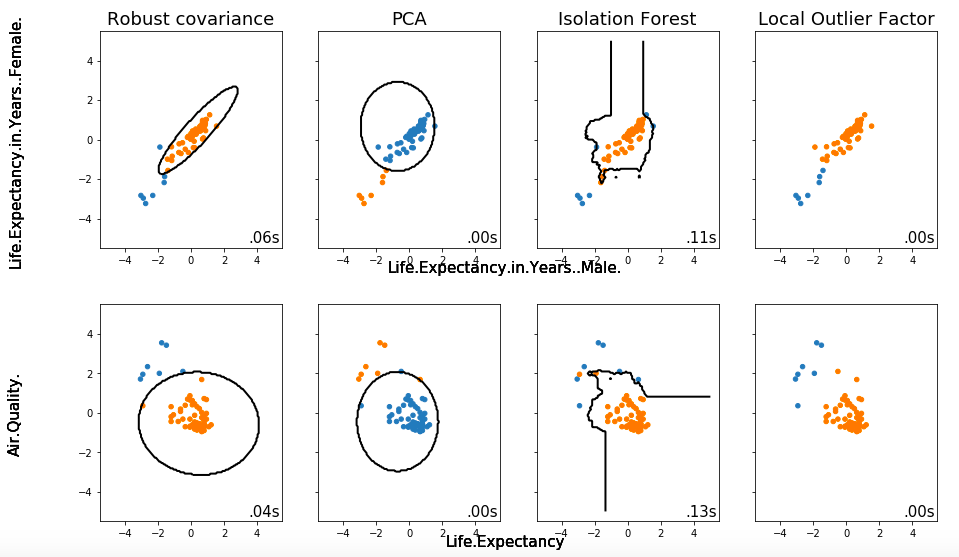
\includegraphics[width=\textwidth]{ADOA/Images/Allcomp1.png}

  %  \caption{Illustration des performences des méthodes: KNN, PCA, Isolation forest and LOF}\hrule
  %  \label{fig6}
%\end{figure*}
%\subsection{Contrôle de qualité}
%\subsection{Finance}





\afterpage{\FloatBarrier}